\chapter{Introduction}
Radiology is an essential part of modern clinical medicine, constituting 10.6\% of health care spending and is virtually ubiquitous in every part of health care \cite{Dodoo:tg}.
Though an indispensable part of the diagnostic workup, the practice of radiology is still fraught with error due to the inherently subjective nature of the task; the doctor must still visually scan, detect, and interpret the findings in the image to deliver an impression. 
An unfortunate consequence of such a system is substantial variability in practice and performance. This dissertation aims to tackle these shortcomings. 
To do so, I propose a novel computational decision-support paradigm aimed at improving the quality and content of the radiological \emph{report} rather than the traditional approaches aimed at directly improving the diagnosis. 
I develop informatics methods within this paradigm to detect and reduce error in reports, and show how these methods have the potential to improve overall diagnostic performance. 
This chapter provides an overview of the dissertation. 
I begin by providing a brief background of radiological error, decision-support systems, and reporting. 
I then give a high-level description of my proposed decision-support model, methods, and key results. 
Finally, I delineate my contributions to the field and provide a guide to the reader for the remainder of the document.

\section{Radiology, variability, and errors}
In its simplest form, radiology is the practice of interpreting medical images. 
Radiologists are presented with functional and/or anatomical images in order to produce an interpretation in the form of a report. 
Though a seemingly straightforward task, the field is fraught with error and variability in performance \cite{Fitzgerald:2001hn} stemming from inadequate imaging techniques \cite{Berlin:1996ib}, poor background knowledge \cite{Berlin:1996ei}, perceptual errors \cite{Berlin:1_mkt9li}, and errors in judgment \cite{Berlin:1996vw}.
Improved work flow and modality research aim to improve imaging techniques \cite{Noumeir:2006cb}, digital imaging and picture archiving and communications systems resolve problems with information transfer to the clinician \cite{Strickland:2000cv,Bryan:1999kn}, computer-aided detection systems aid with identification of lesions in images \cite{Oliver:2010fm}, but to date, there are no wide-spread, commercial tools for improving interpretation.
Errors in judgment are especially pernicious because they are inherent to the subjectivity of qualitative decision-making.
Furthermore, they present a severe detriment to the field; \citeA{Robinson:1997uq} went so far as to state that ``errors and variations in interpretation now represent the weakest aspect of clinical imaging'' and declared such issues ``Radiology's Achilles' heel''. 
This is not to say that radiologists are the only doctors faced with these issues, as the now infamous Institute of Medicine report \emph{To Err is Human: Building a Safer Health System} revealed a striking amount of poor patient outcomes are a result of medical error \cite{Anonymous:2000va}.
A prominent recommendation from this study is the use of automation and computation to improve upon standard of care via decision support systems.

\section{Radiological decision support}
Clinical decision support systems provide assistance to medical care providers with clinical decision-making tasks, typically by assisting with the analysis of complex medical information.
Radiology is a data-rich domain incorporating patient history drawn from the electronic medical record, the patient images, and the reports generated by the radiologists.
As a result, it is a ripe for decision support to assist in organizing, analyzing, and synthesizing these data sources.
Radiological data mining allows clinicians to query similar cases to the ones they are evaluating \cite{Shin:2015wl,Bozkurt:2014jw,Depeursinge:2012ce,Korenblum:2011gx,Akgul:2011ey,Nassif:2009du}.
Computer-aided detection (CADe) systems assist in identifying abnormalities in images across a variety of radiological domains such as mammography, colonoscopy, lung screening, and liver diagnosis \cite{Cheng:2003ig,Castellino:2005ke,Meeuwis:2010bv,Oliver:2010fm,Fenton:2011fw,Fenton:2012kz,Jamieson:2012hz,Gallas:2012eg,Giger:2013jb}.
Computer-aided diagnosis (CADx) systems assist in interpretation of abnormalities found in the image \cite{Jiang:1999fj,ElizabethS:2005gc,Gallas:2012eg,Bright:2012ga,Giger:2013jb,Depeursinge:2010jl,Fujita:2008it,Eadie:2011cv,Rubin:2005jg,Garg:2005cb,Elter:2009fv,Jamieson:2010vl,Jamieson:2010tt,Cheng:2003ig,Jiang:2001fy} as well as interpretation of the content within the radiology report \cite{Burnside:2000wl,ElizabethS:2005gc,Burnside:2009br,Rubin:2005jg}.
Despite these significant technological achievements, adoption of radiological decision support systems is limited.
To date, the only commercially deployed radiological decision support systems are for computer-aided detection (CADe).

Several studies on decision support in radiology show that these systems often interrupt clinical  work-flow, give assessments rather than recommendations, and fail to provide decision-support during decision-making \cite{Kawamoto:2005gn,Morgan:2011ct}.
In general, they still follow the the so-called \emph{Greek Oracle} model of decision support, where the radiologist simply inputs information to a system so that it may make a final decision \cite{Miller:1990wg,Miller:1994cx}.
Such systems fail when deployed in practice since they are based on the implicit assumption that computers can perform the duties of doctors better than doctors themselves.
\citeA{Friedman:2009dx} goes so far as to declare that the \emph{Fundamental Theorem of Biomedical Informatics} is that decision support should ``augment human reasoning'' beyond the capabilities of an unaided practitioner.
Thus, it is crucial to develop radiological decision support tools that fit into the work-flow and augment their reasoning.
The window to provide this support is when radiologists are making their interpretations, which is precisely during reporting \cite{Noumeir:2006cb}.
Yet, \citeA{Reiner:2009ib} states that ``to date, one could argue that effective workflow-enhancing technology does not exist for reporting.''
This insight is a novel contribution to the field of radiological decision support.



\section{Radiology reporting}
The radiology report conveys the radiologist's findings, interpretation of these findings, and suggested patient management \cite{Langlotz:2015vq}.
It is also the primary form of communication of this information to referring clinicians or patients \cite{Sistrom:2005cx}.
Given that communication breakdowns constitute 80\% of medical malpractice lawsuits \cite{Levinson:1994ko}, and radiological reports are legally admissible court documents \cite{Oppenheim:2012tq}, the community has made considerable effort to improve reports \cite{Langlotz:2015vq}.

* errors in reports
* efforts to resolve them via terminology
*where they fall short

Efforts to improve terminology 
The Breast Imaging Reporting and Data System (BI-RADS) successfully standardized the language and assessment guidelines for mammography \cite{Liberman:ws,Langlotz:2009fn,Burnside:2009ki}.
RadLex is an effort to extend this work to all radiological domains by defining a standard radiological lexicon \cite{Langlotz:2006jn}.
Beyond terminology, there is a strong push to create \emph{structured reports} that standardize report format and organization \cite{Langlotz:2009dd,Reiner:2009ib}.
Structured reports not only can improve communication, but they allow for computability of the report information beyond the constraints of free-text documents.
Unfortunately, structured reporting is not without its drawbacks.
It requires new software to implement into the clinical work flow which is costly in terms of integration and training.
More importantly, structured report creation is time-intensive and imposes distractions in the traditional radiological work flow, directly interfering with timeliness \cite{Weiss:2008er}.
Despite these shortcomings, structured reporting is widely seen as the future of radiological reporting \cite{Langlotz:2015vq}.

Both standardized terminology and structured reporting are solid steps to improving the language and format of the report, but they do not go far enough to improve the actual information content in the report.
Several reviews of medical practitioners identify key tenets of report quality that are not addressed by current reporting tools: \textbf{correctness} of findings within the image, \textbf{completeness} of the description of such findings, and \textbf{consistency} of report findings with diagnosis \cite{Johnson:2004kh, HaraldO:2004hi, Reiner:2006fa}.
In the framework of the semiotic triangle, we need to go beyond tools to simply enforce syntax; we need to create methods to improve the \emph{semantic} meaning behind concepts in the report \cite{Mead:2006wm}.
I put forth that decision support systems can provide this level of analysis. 


\section{Providing decision support during reporting time}

\emph{My hypothesis is that delivering decision support during reporting time to improve completeness and correctness of reports will improve consistency, and therefore, diagnostic performance.} To this end, I seek to answer the following questions:

\begin{description}
	\item[How can we improve the quality of the radiological report?] \hfill \\
	Though I have described prior work that aims to improve the terminology and format of the report, there is much to be done to improve upon the \emph{content} of the report. What can we do to improve upon this information? How can we actually implement such solutions?
	
	\item[Does improving the report improve diagnostic performance?] \hfill \\
	There are no studies showing that improving the content of the radiological report can actually improve the diagnostic performance of the physician. If we implement new methods to improve the report, will they have any effect on the radiologist's outcome? Otherwise, are we needlessly burdening radiologists with technology to fix reporting for its own sake?
		
\end{description}


\subsection{Specific Aims}

I answered the hypothesis and questions above by completing the follow three specific aims:

\begin{enumerate}
	\item \textbf{Developed methods to assess completeness and correctness of radiology reports}
	
	I proposed metrics to measure completeness and correctness of radiology reports. Then I present methods to calculate these metrics in an efficient and reproducible manner.
	
	\item \textbf{Evaluated these methods in two important radiological domains (mammography and liver CT)}
	
	I showed that the correctness metric has good accuracy in automatically annotating radiological images. I also show that the completeness metric is clinically significant by correlating it with error in interpretation.
	
	\item \textbf{Developed framework to provide feedback to radiologist to ensure consistency between report and diagnosis, improving diagnostic performance}
	
	I developed a framework for providing feedback to radiologists to improve their reports and show that this framework can improve the performance of existing decision support systems.
\end{enumerate}

\subsection{Methodology}

\begin{figure}[h]
	\centering
	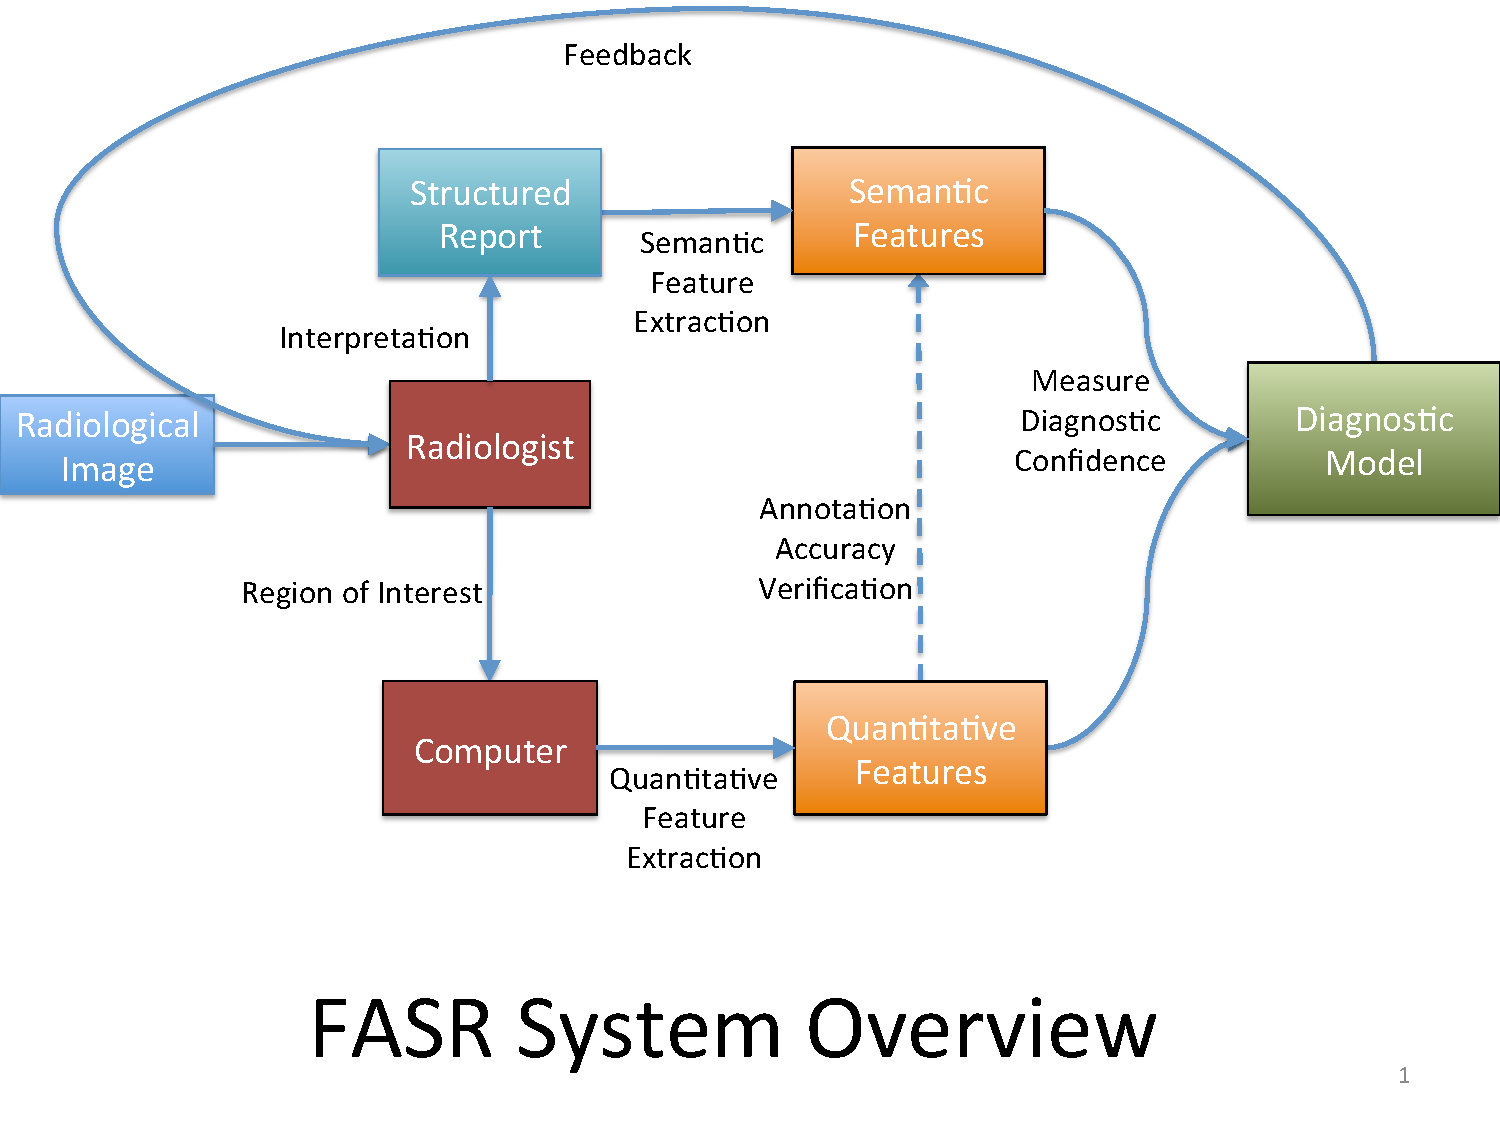
\includegraphics[width=1\linewidth]{fasr_diagram.pdf}
	\caption[Overview of the Fast Adaptive Structured Reporting (FASR) system]{The Fast Adaptive Structured Reporting System (FASR) plugs into the traditional radiological workflow but concurrently analyzing the image and information in the radiology report while the radiologists performs their interpretation. It then provides checks for completeness, correctness, and consistency.}
	\label{fig:fasr_diagram}
\end{figure}

I propose Fast Adaptive Structured Reporting (FASR), a real-time decision support system that provides feedback to radiologists as they generate their reports. This system enables the translation of decision support systems into clinical practice to benefit patient care. To do so, it plugs directly into the existing reporting work flow and performs analysis in parallel to the radiologist.

Figure \ref{fig:fasr_diagram} shows the work flow of the FASR system. An image is sent to a radiologist who identifies an abnormality and delineates it. Then, while the radiologist creates the structured report, the computer analyzes the image. When the radiologist finishes their report, the system will compare the radiologist's output to its predicted output. If they disagree, it triggers a warning that a descriptor may be incomplete. Upon finishing this check, FASR then looks at the information content of the radiology report in conjunction with the diagnosis made by the radiologist. Should the information content of the report lack a complete description of the image phenotype the system will alert the radiologist. Finally, it checks if there is consistency between the image descriptors and diagnosis. If they are discordant, a feedback system requests more information of the radiologist to clarify the diagnosis.

\subsection{Key Results}

I conducted several studies to develop, implement, and evaluate the main components in the FASR system. Here I present the key results, with more details in chapters 3, 4, and 5. 

\begin{description}
	\item[Can computational methods correct report observations?] \hfill \\
	I posed this task as a supervised classification problem to predict the radiologist observations about liver lesions in CT scans. I show that it is possible to accurately predict salient report observations, with a mean misclassification rate of $0.144\pm0.09$ and AUC of $0.816\pm0.141$ across 30 different observation tasks. These results suggest that it is feasible to use computational image analysis as a ``second reader'' for images.
	
	\item[How do we measure the completeness of reporting content?] \hfill \\
	I used a decision-theoretic approach to quantify completeness of information. I do so by defining \emph{incompleteness score} as the probability that the clinical decision changes if missing information in the report were to be observed. I calculated this value on 3,695 mammography reports, and found that the incompleteness score was ~10x higher for reports with errors (incompleteness = 0.072) than reports that were correct (incompleteness = 0.0079). These results are the first to show that poor reporting is indicative of diagnostic error.
	
	\item[Does enforcing consistency improve diagnostic performance?] \hfill \\
	I developed a framework that enforces consistency between report content and diagnosis by estimating the accuracy of follow-up decisions given current observations, and requesting more observations if there is a discrepancy between the two. I evaluate this framework in a set of generated mammography reports by using it to request observations from simulated radiologists who provide feedback. I show that a decision support system that intelligently requests a subset of meaningful observations can achieve better performance (accuracy = 0.936, mean observations = 4.0) than a system that has access to \emph{all} possible observations (accuracy = 0.921, mean observations = 20). This result shows that efficient reporting is not only achievable but actually more desirable with respect to performance.
\end{description}

\section{Summary of contributions}
This work demonstrates contributions to our understanding of reporting in radiology as well as performance of decision-support systems for diagnostics.

\subsection{Radiology contributions}

\begin{itemize}
	\item I developed a system to automatically annotate liver lesions with their radiological descriptors via image processing and machine learning. Showed how this system could verify correctness of observations.
	\item I was the first to quantify completeness of radiological reports and showed that incomplete reports are correlated with errors in diagnosis.
\end{itemize}

\subsection{Informatics Contributions}

\begin{itemize}
	\item Showed how to perform semantic annotations of images by extracting high dimensionality features and using regularized models for prediction.
	\item Developed a new Monte-Carlo algorithm to approximate the computationally intractable same-decision probability measure in Bayesian networks.
	\item Formalized a framework for delivering feedback in decision-support systems that allows for evaluation based on diagnostic performance.
\end{itemize}


\section{Guide for the reader}
This dissertation covers the novel methods I have developed for the FASR system to improve correctness, completeness, and consistency in radiology reports. The following chapters go into detail about the problems, solutions, and evaluations I have described in this introduction. \textbf{Chapter 2} provides a background of challenges in radiology and prior methods to attack them using decision support. These works have been extremely valuable and influential for my own methodological development. In \textbf{chapter 3} I describe my method to perform automatic annotation of images with radiological descriptors and then describe how it can be used to correct mistakes in reports. In \textbf{chapter 4} I define a new measure for information content in radiology reports to quantify how complete they are and provide a new algorithm to compute this score. I also show some clinical consequences of incomplete reporting. In \textbf{chapter 5} I formulate a framework to provide feedback to radiologists when we have discovered errors in their reports. I show that this framework can significantly improve computer-aided diagnostic systems by incorporating human feedback. Finally, in \textbf{chapter 6} I provide some concluding remarks, limitations, and future work for this field.